% !TeX spellcheck = en_GB
\section{Conclusion}
%\subsection{Summary}
We have studied percolation fractals in the most general form (starting from a $D$ dimensional cuboid).
Classical percolations almost surely have the same dimension as the initial set\footnotemark, while recursive percolations have almost sure dimension in $\left[ 0, D \right)$
\addtocounter{footnote}{-1}
\footnotemark
\footnotetext{For $p \in \left( 0,1 \right)$.}.
We have proved that recursive percolations reach a density of zero eventually, almost surely.
Moreover, they are totally disconnected when $p$ is small enough\footnote{When $p \leq \nicefrac{1}{\sqrt{n^{D-1}}}$.}.

We also studied the probability of the existence of a crossing.
It in fact has a physical motivation: if the percolation represents a porous material, the presence of a crossing tells if it is fluid-proof.
The complexity of this problem pushed us to make numerical simulations.
We reduced our study to cases in two and three dimensions, and developed efficient algorithms to get the most reliable results (by increasing the number of experiments)\footnote{All results are aggregated at \url{https://pauldubois98.github.io/PercolationFractalsStudy/}.}.

%\subsection{Future Work}
In the future, it could be interesting to examine the dimensionality of the crossing path.
We anticipate the dimension will be one when the path is nearly straight, but this may increase for a more irregular paths.
The dimension of the path could be a good measure of the physical difficulty for a fluid to traverse the material.
This, together with the viscosity of the fluid could be interpreted as the strength of fluid flow traversing the medium.

It would also be interesting to see the effect of removing other shapes from the initial cuboid.
Many porous materials have round (or spherical) holes.
It would therefore make sense to study percolations where the set removed is a $D$ dimensional ball, rather than a $D$ dimensional cuboid, as we have done so far.
This would make the model more complicated, but also more accurate in terms of physical interpretation (see fig. \ref{fig:porousModels}).

\begin{figure}[!h]
	\vspace{4cm}
	\begin{subfigure}{0.44\linewidth}
		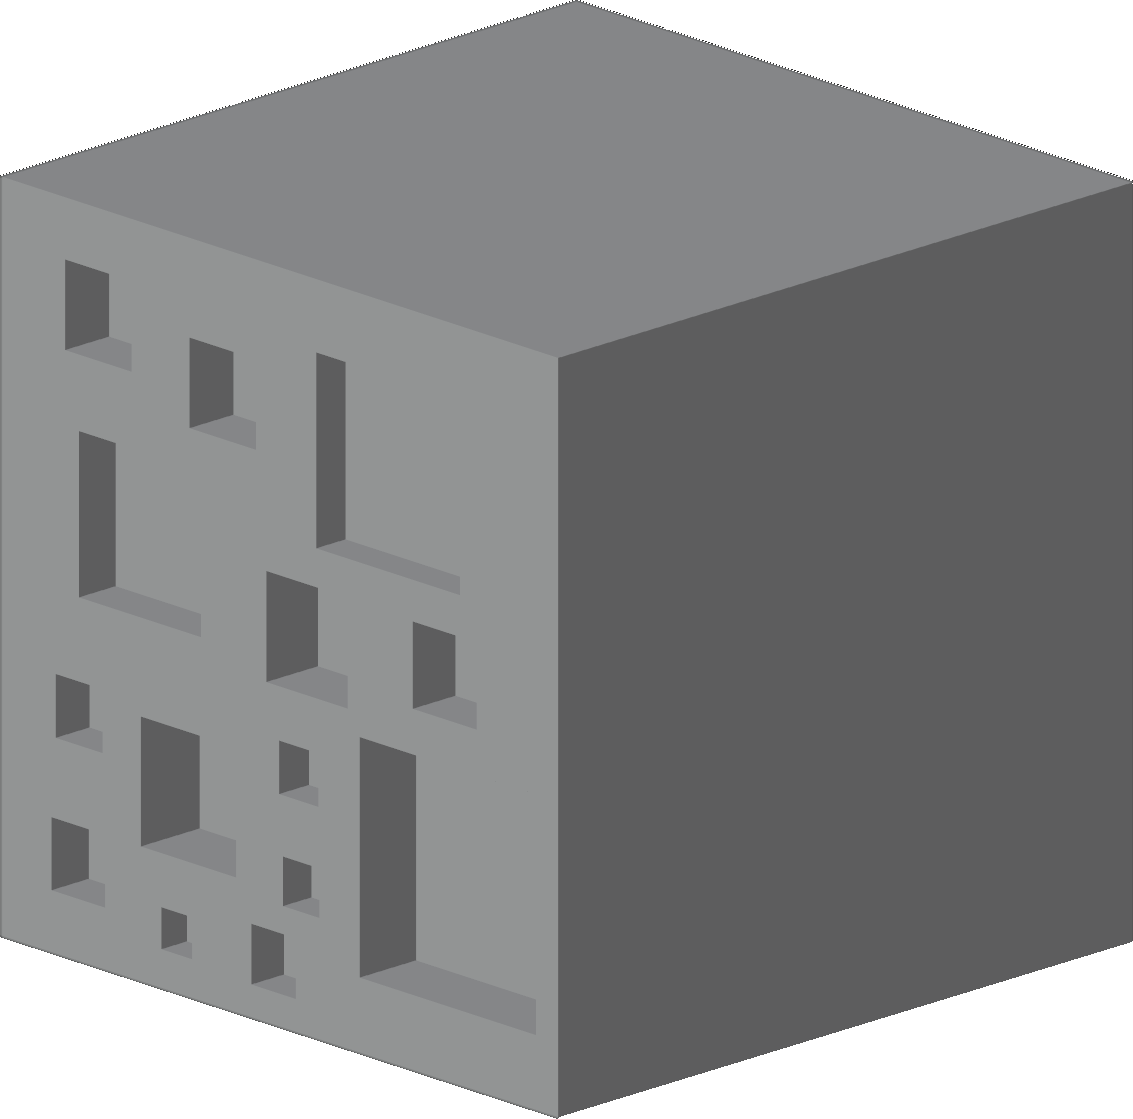
\includegraphics[width=5.25cm]{porousModelCuboids}
		\centering
		\captionsetup{justification=centering}
		\caption{Porous material with cubic (3 dimensional cuboids) holes.}
		\label{fig:porousModelCuboids}
	\end{subfigure}
	\hspace{0.1\linewidth}
	\begin{subfigure}{0.44\linewidth}
		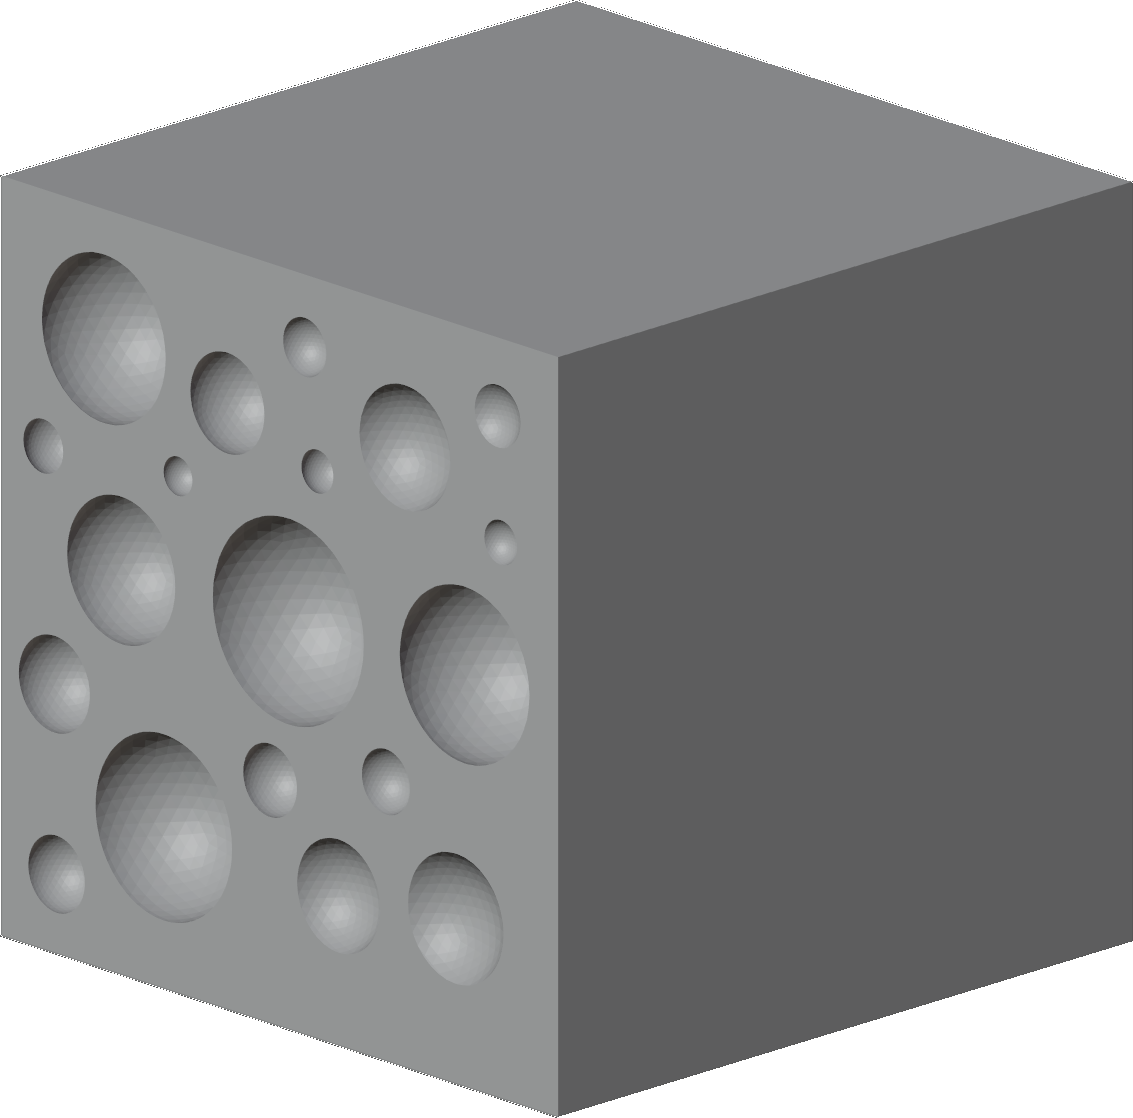
\includegraphics[width=5.25cm]{porousModelBalls}
		\centering
		\captionsetup{justification=centering}
		\caption{Porous material with spherical (3 dimensional balls) holes.}
		\label{fig:porousModelBalls}
	\end{subfigure}
	\centering
	\caption{Porous materials are more realistically modelled with spherical holes than cubic holes.}
	\label{fig:porousModels}
\end{figure}
